\subsection{BÀI TẬP TRẮC NGHIỆM}
\setcounter{ex}{0}

\ind{PHẦN I.} \inden{Câu trắc nghiệm nhiều phương án lựa chọn. Học sinh trả lời từ câu 1 đến câu 20. Mỗi câu hỏi học sinh chỉ chọn một phương án.}\\
\setcounter{ex}{0}
\Opensolutionfile{ans}[ans/1D1-B4-1]
\begin{ex}%[1D1Y2]
	Phương trình nào sau đây vô nghiệm?
	\choice
	{$\sin x=\dfrac{1}{2}$}
	{$\tan x=\sqrt{3}$}
	{\True $\sin x=3$}
	{$\cos x=-\dfrac{1}{2}$}
	\loigiai{
	Phương trình $\sin x =a$ có nghiệm khi $a \in [-1;1]$ nên phương trình $\sin x=3$ vô nghiệm}
\end{ex}\cham{4}

\begin{ex}%[1D1Y2]
	Nghiệm của phương trình $\sin x=-1$ là
	\choice
	{$x=-\dfrac{\pi}{2}+k\pi,k\in\mathbb{Z}$}
	{$x=k\pi,k\in\mathbb{Z}$}
	{$x=\dfrac{3\pi}{2}+k\pi,k\in\mathbb{Z}$}
	{\True $x=-\dfrac{\pi}{2}+k2\pi,k\in\mathbb{Z}$}
	\loigiai{
		Ta có $\sin x=-1\Leftrightarrow\sin x=\sin \dfrac{-\pi}{2}\Leftrightarrow x=\dfrac{-\pi}{2}+k2\pi,k\in\mathbb{Z}$.
	}
\end{ex}\cham{4}

\begin{ex}%[1D1Y2]
	Tìm tất cả các nghiệm của phương trình $\sin3x =\dfrac{\sqrt{3}}{2}$.
	\choice
	{\True $\hoac{&x =\dfrac{\pi}{9} + \dfrac{k2\pi}{3},\ k \in\mathbb{Z}\\&x =\dfrac{2\pi}{9} + \dfrac{k2\pi}{3},\ k \in\mathbb{Z}}$}
	{$\hoac{&x =\dfrac{\pi}{9} + k2\pi ,\ k \in\mathbb{Z}\\&x =\dfrac{2\pi}{9} + k2\pi ,\ k \in\mathbb{Z}}$}
	{$\hoac{&x =\dfrac{\pi}{9} + \dfrac{k\pi}{3},\ k \in\mathbb{Z}\\&x =\dfrac{2\pi}{9} + \dfrac{k\pi}{3},\ k \in\mathbb{Z}}$}
	{$\hoac{&x =\dfrac{\pi}{3} + \dfrac{k2\pi}{3},\ k \in\mathbb{Z}\\&x =\dfrac{2\pi}{3} + \dfrac{k2\pi}{3},\ k \in\mathbb{Z}}$}
	\loigiai{
		$\sin3x = \dfrac{\sqrt{3}}{2} \Leftrightarrow \hoac{&3x = \dfrac{\pi}{3} + k2\pi ,\ k \in\mathbb{Z}\\&3x = \dfrac{2\pi}{3} + k2\pi ,\ k \in\mathbb{Z}
		} \Leftrightarrow \hoac{&x = \dfrac{\pi}{9} + \dfrac{{k2\pi }}{3},\ k \in\mathbb{Z}\\&x = \dfrac{2\pi}{9} + \dfrac{{k2\pi }}{3},\ k \in\mathbb{Z}}$.
	}
\end{ex}\cham{5}

\begin{ex}%[1D1B2]
	Nghiệm của phương trình $2\sin x+1=0$ là
	\choice
	{$x=\dfrac{11\pi}{6}+k2\pi $ và $x=\dfrac{-\pi}{6}+k2\pi $}
	{$x=\dfrac{\pi}{6}+k2\pi $ và $x=\dfrac{-7\pi}{6}+k2\pi $}
	{$x=\dfrac{-\pi}{6}+k\pi $ và $x=\dfrac{7\pi}{6}+k\pi $}
	{\True $x=\dfrac{-\pi}{6}+k2\pi $ và $x=\dfrac{7\pi}{6}+k2\pi$}
	\loigiai{
		$2\sin x +1 =0 \Leftrightarrow \sin x=-\dfrac{1}{2} \Leftrightarrow \sin x =\sin \left(-\dfrac{\pi}{6}\right) \Leftrightarrow x=-\dfrac{\pi}{6}+k2\pi $ và $x=\dfrac{7\pi}{6}+k2\pi$}
\end{ex}\cham{5}

\begin{ex}%[1D1B2]
	Tập nghiệm của phương trình $\sin2x=1$ là
	\choice
	{$\left\{\dfrac{\pi}{4}+2k\pi,k\in\mathbb{Z}\right\}$}
	{\True $\left\{\dfrac{\pi}{4}+k\pi,k\in\mathbb{Z}\right\}$}
	{$\left\{k\pi,k\in\mathbb{Z}\right\}$}
	{$\left\{\dfrac{\pi}{2}+2k\pi,k\in\mathbb{Z}\right\}$}
\end{ex}\cham{4}

\begin{ex}%[1D1Y2]
	Phương trình $ \cos x=-\dfrac{\sqrt{3}}{2} $ có tập nghiệm là
	\choice
	{\True $\left\{x=\pm \dfrac{5\pi}{6}+k2\pi; k\in \mathbb{Z} \right\}$}
	{$\left\{x=\pm \dfrac{\pi}{3}+k\pi; k\in \mathbb{Z} \right\}$}
	{$\left\{x=\pm \dfrac{\pi}{3}+k2\pi; k\in \mathbb{Z} \right\}$}
	{$\left\{x=\pm \dfrac{\pi}{6}+k\pi; k\in \mathbb{Z} \right\}$}
	\loigiai{
		Ta có $ \cos x=-\dfrac{\sqrt{3}}{2}\Leftrightarrow \cos x =\cos \left(\dfrac{5\pi}{6}\right)\Leftrightarrow x=\pm \dfrac{5\pi}{6}+k2\pi; k\in \mathbb{Z}. $
	}
\end{ex}\cham{7}

\begin{ex}
	Tập nghiệm của phương trình $\cos 2x = -1$ là
	\choice
	{$-k\pi, k \in \mathbb{Z}$}
	{$\left\{-\dfrac{\pi}{4} + k\pi, k \in \mathbb{Z}\right\}$}
	{$\left\{-\dfrac{\pi}{2} + k2\pi, k \in \mathbb{Z}\right\}$}
	{\True $\left\{90^\circ + k180^\circ, k \in \mathbb{Z}\right\}$}
	\loigiai{
		Ta có:
		$$ \cos 2x = -1 \Leftrightarrow 2x = 180^\circ + k360^\circ \Leftrightarrow x = 90^\circ + k180^\circ \ (k \in \mathbb{Z}). $$
		Vậy tập nghiệm của phương trình là $\left\{90^\circ + k180^\circ, k \in \mathbb{Z}\right\}$.
	}
\end{ex}\cham{6}

\begin{ex}%[1D1B2]
	Phương trình $2\cos x-1=0$ có nghiệm là
	\choice
	{$x=\pm \dfrac{\pi}{6}+k2\pi$, $k\in \mathbb{Z}$}
	{$x=\pm \dfrac{\pi}{3}+k\pi$, $k\in \mathbb{Z}$}
	{$x=\pm \dfrac{\pi}{6}+2\pi$, $k\in \mathbb{Z}$}
	{\True $x=\pm \dfrac{\pi}{3}+k2\pi$, $k\in \mathbb{Z}$}
	\loigiai{
		$2\cos x-1=0 \Leftrightarrow \cos x=\dfrac{1}{2} \Leftrightarrow x=\pm \dfrac{\pi}{3}+k2\pi$, $k\in \mathbb{Z}$.
	}
\end{ex}\cham{6}

\begin{ex}%[1D1B2]
	Số nghiệm của phương trình $2\cos\left(x-\dfrac{\pi}{2}\right)=1$ trong khoảng $(0;\pi)$ là
	\choice
	{4}
	{1}
	{\True 2}
	{3}
	\loigiai{
	}
\end{ex}\cham{7}

\begin{ex}%[1D1B2-1]
	Phương trình $\sin x-\cos x=1$ có một nghiệm là
	\choice
	{$-\dfrac{\pi}{2}$}
	{$\dfrac{\pi}{4}$}
	{$\dfrac{2\pi}{3}$}
	{\True $\pi $}
	\loigiai{
		Ta có
		\begin{eqnarray*}
			&& \sin x-\cos x=1 \Leftrightarrow \sin \left(x-\dfrac{\pi}{4}\right)=\dfrac{1}{\sqrt{2}} \\
			&\Leftrightarrow &
			\hoac{& x-\dfrac{\pi}{4}=\dfrac{\pi}{4}+k2\pi \\& x-\dfrac{\pi}{4}=\pi -\dfrac{\pi}{4}+k2\pi} \Leftrightarrow
			\hoac{& x=\dfrac{\pi}{2}+k2\pi \\& x=\pi +k2\pi}(k\in\mathbb{R}).
		\end{eqnarray*}
		Vậy phương trình đã cho có một nghiệm là $x=\pi $.
	}
\end{ex}\cham{7}

\begin{ex}%[1D1K2]
	Nghiệm của phương trình $\sin^4 x-\cos^4x=0$ là
	\choice
	{$x=\pi+k2\pi$}
	{$x=k\pi$}
	{$x=\dfrac{\pi}{2}+k\pi$}
	{\True $x=\dfrac{\pi}{4}+k\dfrac{\pi}{2}$}
	\loigiai{
		$\sin^4 x - \cos^4 x=0\Leftrightarrow \left(\sin^2 x + \cos^2 x \right)\left( \sin^2 x - \cos^2 x\right)=0\\
		\Leftrightarrow -\cos {2x}=0\Leftrightarrow 2x=\dfrac{\pi}{2}+k\pi \Leftrightarrow x= \dfrac{\pi}{4}+k\dfrac{\pi}{2}$, $k\in \mathbb{Z}$.
	}
\end{ex}\cham{7}

\begin{ex}%[1D1B2]
	Xét trên $\left({-\pi ; \pi}\right)$,  phương trình $ \sin x = \dfrac{2}{3} $ có bao nhiêu nghiệm?
	\choice
	{1}
	{3}
	{\True 2}
	{4}
	\loigiai{
		$ \sin x = \dfrac{2}{3} \Leftrightarrow x=\arcsin\frac{2}{3}+k2\pi$ và $x=\pi-\arcsin\frac{2}{3}+k2\pi$.\\
		Xét trên $\left({-\pi ; \pi}\right)$ thì ta được hai nghiệm là $x=\arcsin\frac{2}{3}$ và $x=\pi-\arcsin\frac{2}{3}$.
	}
\end{ex}\cham{7}

\begin{ex}%[1D1B2-1]
	Cho phương trình $\sin 2x = \dfrac{\sqrt{3}}{2}$. Gọi $n$ là số các nghiệm của phương trình trong đoạn $\left[0; 3\pi\right]$ thì giá trị của $n$ là
	\choice
	{$n = 8$}
	{$n = 5$}
	{\True $n = 6$}
	{$n = 2$}
	\loigiai{
		Ta có
		\begin{align*}
			\sin 2x = \dfrac{\sqrt{3}}{2} &\Leftrightarrow \sin 2x = \sin \dfrac{\pi}{3}\\
			& \Leftrightarrow \hoac{& 2x = \dfrac{\pi}{3} + k2\pi\\& 2x = \dfrac{2\pi}{3} + k2\pi}\\
			& \Leftrightarrow \hoac{& x = \dfrac{\pi}{6} + k\pi\\& x = \dfrac{\pi}{3} + k\pi.}
		\end{align*}
		Xét trên đoạn $\left[0; 3\pi\right]$ có tất cả $6$ nghiệm là $x = \left\lbrace \dfrac{\pi}{6}, \dfrac{7\pi}{6}, \dfrac{13\pi}{6}, \dfrac{\pi}{3}, \dfrac{4\pi}{3}, \dfrac{7\pi}{3}\right\rbrace $.
	}
\end{ex}\cham{7}

\begin{ex}%[1D1K2-1]
	Tính tổng các nghiệm $x\in [0;2018\pi ]$ của phương trình $\sin 2x=1$.
	\choice
	{\True $S=\dfrac {4071315\pi}{2}$}
	{$S=\dfrac {4071315\pi}{4}$}
	{$S=\dfrac {8141621\pi}{2}$}
	{$S=\dfrac {8141621\pi}{4}$}
	\loigiai{
		$\sin 2x=1\Leftrightarrow x=\dfrac {\pi}{4}+k\pi$, $k\in \mathbb{Z}$.\\
		Do $x\in [0;2018\pi ]$ nên $0\le \dfrac {\pi}{4}+k\pi \le 2018\pi \Leftrightarrow -0{,}25\le k\le 2017{,}75$.\\
		Các nghiệm của phương trình lượng giác lập thành một cấp số cộng với số hạng đầu ứng với $k=0$ và số hạng cuối ứng với $k=2017$.\\
		Bấm máy: $\displaystyle \sum\limits_{x=0}^{2017}{\left(\dfrac {\pi}{4}+x\pi \right)}$, ta được kết quả  $\dfrac {4071315\pi}{2}$.}
\end{ex}\cham{7}

\begin{ex}%[1D1K2-1]
	Tìm số nghiệm thuộc khoảng $\left(-\pi;\pi \right)$ của phương trình $\cos x+\sin 2x=0$
	\choice
	{$1$}
	{\True $4$}
	{$2$}
	{$3$}
	\loigiai{
		$\cos x+\sin 2x=0 \Leftrightarrow \cos x = \sin(-2x) \Leftrightarrow \cos x = \cos \left( \dfrac{\pi}{2}+2x \right)\Leftrightarrow \hoac{&x=-\dfrac{\pi}{2}+k2 \pi\\& x=-\dfrac{\pi}{6}+k\dfrac{2\pi}{3}} \; (k\in \mathbb{Z})$.\\
		Vì $x\in \left(-\pi;\pi \right)$ nên ta có các nghiệm $-\dfrac{\pi}{2};-\dfrac{\pi}{6};-\dfrac{5\pi}{6};\dfrac{\pi}{2}$.
	}
\end{ex}\cham{6}

\begin{ex}%[1D1G2-1]
	Phương trình $\sin 5x - \sin x = 0$ có bao nhiêu nghiệm thuộc đoạn $\left[-2018\pi ;2018\pi \right]$?
	\choice
	{\True $16145$}
	{$20181$}
	{$20179$}
	{$16144$}
	\loigiai{
		Ta có
		\begin{eqnarray*}
			& \sin 5x-\sin x=0 & \Leftrightarrow \sin 5x=\sin x \\
			& & \Leftrightarrow \left[\begin{aligned}
				&5x=x+k2\pi \\
				&5x=\pi -x+k2\pi
			\end{aligned}\right.\\
			& & \Leftrightarrow \left[\begin{aligned}
				&x=k\dfrac{\pi}{2} \\
				&x=\dfrac{\pi}{6}+k\dfrac{\pi}{3}
			\end{aligned}\right. \\
			& & \Leftrightarrow \left[\begin{aligned}
				&x=k\dfrac{\pi}{2} & \left(k\in \mathbb{Z}\right) \\
				&x=\dfrac{5\pi}{6}+m\pi & \left(m\in \mathbb{Z}\right) \\
				&x=\dfrac{\pi}{6}+n\pi & \left(n\in \mathbb{Z}\right).
			\end{aligned}\right.
		\end{eqnarray*}
		Vì $x\in \left[-2018\pi;2018\pi \right]$ nên $\left\{\begin{aligned}
			&-2018\pi \leq k\dfrac{\pi}{2}\leq 2018\pi \\
			&-2018\pi \leq \dfrac{5\pi}{6}+m\pi \leq 2018\pi \\
			&-2018\pi \leq \dfrac{\pi}{6}+n\pi \leq 2018\pi
		\end{aligned}\right. $ $ \Leftrightarrow \left\{\begin{aligned}
			&-4036\leq k\leq 4036 \\
			&-\dfrac{12113}{6}\leq m\leq \dfrac{12103}{6} \\
			&-\dfrac{12109}{6}\leq n\leq \dfrac{12107}{6}
		\end{aligned}\right. $.
		Do đó có $8073$ giá trị $k$, $4036$ giá trị $m$, $4036$ giá trị $n$, suy ra số nghiêm cần tìm là $16145$ nghiệm.
	}
\end{ex}\cham{7}

\begin{ex}
	Đồ thị của các hàm số $y=\sin x$ và $y=\cos x$ cắt nhau tại bao nhiêu điểm có hoành độ thuộc đoạn $\left[-2 \pi ; \dfrac{5 \pi}{2}\right]$?
	\choice
	{\True 5}
	{6}
	{4}
	{7}
	\loigiai{
		Xét phương trình hoành độ giao điểm $$\sin x = \cos x \Leftrightarrow \tan x =1 \Leftrightarrow x = \dfrac{\pi}{4}+k \pi$$
		Với $$-2\pi \le x \le \dfrac{5 \pi}{2} \Rightarrow -2\pi \le \dfrac{\pi}{4}+k \pi \le \dfrac{5 \pi}{2} \Rightarrow -\dfrac{9}{4} \le k \le \dfrac{9}{4}.$$
		Mà $k \in \mathbb{Z}$ nên $k \in \{-2;-1;0;1;2\}$. Có 5 giá trị thỏa yêu cầu, suy ra hai đồ thị cắt nhau tại 5 điểm.
	}
\end{ex}\cham{7}

\begin{ex}%[1D1Y3-7]%
	Với giá trị của tham số $m$ thì phương trình $\cos\left(x-\dfrac{\pi}{3}\right)-2m=0$ vô nghiệm?
	\choice
	{\True $\hoac{&m<-\dfrac{1}{2}\\&m>\dfrac{1}{2}}$}
	{ $\hoac{&m\le-\dfrac{1}{2}\\&m\ge\dfrac{1}{2}}$}
	{ $\hoac{&m\le-1\\&m\ge1}$}
	{ $\hoac{&m<-1\\&m>1}$}
	\loigiai
	{Ta có: $\cos\left(x-\dfrac{\pi}{3}\right)-2m=0 \Leftrightarrow \cos\left(x-\dfrac{\pi}{3}\right)= 2m$.\\ Để phương trình vô nghiệm khi và chỉ khi $\hoac{&2m<-1\\&2m>1} \Leftrightarrow \hoac{&m<-\dfrac{1}{2}\\&m>\dfrac{1}{2}}$.
	}
\end{ex}\cham{6}

\begin{ex}
	Tìm tất cả các giá trị nguyên của tham số $m$ để phương trình $\cos^2 \pi x=m^2-9$ có nghiệm.
	\choice
	{$5$}
	{\True $2$}
	{$1$ }
	{$3$ }
	\loigiai{
		Do $0 \le \cos^2 \pi x \le 1$ nên $0 \le m^2-9 \le 1$. Chọn được $m=\pm 3$ thỏa mãn.
	}
\end{ex}\cham{7}

\begin{ex}
	Cho vận tốc $v$ (cm/s) của một con lắc đơn theo thời gian $t$ (giây) được cho bởi công thức $v=-3 \sin \left(1,5 t+\dfrac{\pi}{3}\right)$. Xác định các thời điểm $t$ mà tại đó vận tốc con lắc đạt giá trị lớn nhất.
	\choice
	{$t=\dfrac{5\pi}{9}+\dfrac{4 \pi}{3}k, \,\,k \in \mathbb{Z}$}
	{\True $t=\dfrac{7 \pi}{9}+\dfrac{4 \pi}{3}k, \,\,k \in \mathbb{Z}$}
	{$t=\dfrac{8\pi}{9}+\dfrac{4 \pi}{3}k, \,\,k \in \mathbb{Z}$}
	{$t=\dfrac{4\pi}{9}+\dfrac{4 \pi}{3}k, \,\,k \in \mathbb{Z}$}
	\loigiai{
		Vận tốc đạt giá trị lớn nhất khi $\sin \left(1,5 t+\dfrac{\pi}{3}\right)=-1$. \\
		Giải phương trình này, ta được nghiệm $t=\dfrac{7 \pi}{9}+\dfrac{4 \pi}{3}k, \,\,k \in \mathbb{Z}$ }
\end{ex}\cham{7}
\Closesolutionfile{ans}

\ind{PHẦN II.} \inden{Câu trắc nghiệm đúng sai. Học sinh trả lời từ câu 21 đến câu 25. Trong mỗi ý a), b), c), d) ở mỗi câu, học sinh chọn đúng hoặc sai.}\\
\Opensolutionfile{ans}[ans/1D1-B4-2]

\begin{ex}
	Cho phương trình $\cos 2x =0$. Xét tính đúng sai của các khẳng định sau:
	\choiceTF
	{$x=0$ là một nghiệm của phương trình}
	{Nghiệm của phương trình là $x=\dfrac{\pi}{2}+k\pi$, với $k \in \mathbb{Z}$.}
	{\True Phương trình có cùng tập nghiệm với phương trình $\cos^2 x =\dfrac{1}{2}$}
	{Trên $(0;2\pi)$, phương trình có đúng 2 nghiệm}
	\loigiai{
	\begin{itemchoice}
		\itemch  Với $x=0$, ta có $\cos 2x =\cos 2\cdot 0 = \cos 0 =1$. Suy ra $x=0$ không phải là nghiệm của phương trình $\cos 2x =0$.
		\itemch  Xét $\cos 2x =0 \Leftrightarrow 2x =\dfrac{\pi}{2}+k\pi \Leftrightarrow x=\dfrac{\pi}{4}+k\dfrac{\pi}{2}$, với $k \in \mathbb{Z}$.
		\itemch Xét $\cos^2 x =\dfrac{1}{2} \Leftrightarrow 2\cos^2 x =1 \Leftrightarrow 2\cos^2 x -1=0 \Leftrightarrow \cos 2x =0$. Vậy hai phương trình này có cùng tập nghiệm.
		\itemch Ta có $\cos 2x =0 \Leftrightarrow 2x =\dfrac{\pi}{2}+k\pi \Leftrightarrow x=\dfrac{\pi}{4}+k\dfrac{\pi}{2}$.\\
		Với $x \in (0;2\pi)$, suy ra $0<\dfrac{\pi}{4}+k\dfrac{\pi}{2}<2\pi \Leftrightarrow -\dfrac{1}{4}<k<\dfrac{7}{2}$.\\
		Do $k \in \mathbb{Z}$, suy ra $k \in \{0;1;2;3\}$. Mỗi giá trị $k$, ta tìm được 1 nghiệm, nên trên $(0;2\pi)$ phương trình có đúng 4 nghiệm.
	\end{itemchoice}
	}
\end{ex}\cham{8}

\begin{ex}
	Cho phương trình $\sin x = \cos x$. Xét tính đúng sai của các khẳng định sau:
	\choiceTF
	{$x=\dfrac{3\pi}{4}$ là một nghiệm của phương trình}
	{Nghiệm của phương trình là $x=\dfrac{\pi}{2}+k2\pi$, với $k \in \mathbb{Z}$.}
	{\True Phương trình có cùng tập nghiệm với phương trình $\tan x =1$}
	{\True Trên $(0;2\pi)$, phương trình có đúng 2 nghiệm}
	\loigiai{
		\begin{itemchoice}
			\itemch Thay $x=\dfrac{3\pi}{4}$ vào phương trình không thỏa. Suy ra $x=\dfrac{3\pi}{4}$ không là một nghiệm của phương trình.
			\itemch $\sin x = \cos x \Leftrightarrow \dfrac{\sin x}{\cos x}=1 \Leftrightarrow \tan x=1 \Leftrightarrow x=\dfrac{\pi}{4}+k\pi$.
			\itemch $\tan x =1 \Leftrightarrow x=\dfrac{\pi}{4}+k\pi$. Vậy hai phương trình có cùng tập nghiệm.
			\itemch Trên $(0;2\pi)$, ta có đúng hai nghiệm $x=\dfrac{\pi}{4}$, $x=\dfrac{5\pi}{4}$.
		\end{itemchoice}
	}
\end{ex}\cham{10}

\begin{ex}
	Nhiệt độ ngoài trời ở một thành phố vào các thời điểm khác nhau trong ngày có thể được mô phỏng bởi công thức
	$$
	h(t)=29+3\sin\left[\dfrac{\pi}{12}(t-9)\right]
	$$
	với $h$ tính bằng độ $\mathrm{C}$ và $t$ là thời gian trong ngày tính bằng giờ $(0 \le t <24)$. Xét tính đúng sai của các khẳng định sau:
	\choiceTF
	{Nhiệt độ ngoài trời cao nhất bằng 29 $^\circ$C}
	{\True Nhiệt độ ngoài trời thấp nhất bằng 26 $^\circ$C}
	{Nhiệt độ ngoài trời cao nhất vào thời điểm $12$ giờ trưa}
	{\True Nhiệt độ ngoài trời thấp nhất vào thời điểm $3$ giờ sáng} 
	\loigiai{
		\begin{itemchoice}
			\itemch Do $-1 \le \sin\left[\dfrac{\pi}{12}(t-9)\right] \le 1 \Rightarrow 26 \le h(t) \le 32$. \\
			Suy ra, nhiệt độ ngoài trời cao nhất bằng 32 $^\circ$C.
			\itemch Do $-1 \le \sin\left[\dfrac{\pi}{12}(t-9)\right] \le 1 \Rightarrow 26 \le h(t) \le 32$.\\
			 Suy ra, nhiệt độ ngoài trời thấp nhất bằng 26 $^\circ$C.
			\itemch Nhiệt độ ngoài trời cao nhất khi $\sin\left[\dfrac{\pi}{12}(t-9)\right]=1 \Rightarrow t=15$. Vậy nhiệt độ ngoài trời cao nhất vào thời điểm $15$ giờ.
			\itemch Nhiệt độ thấp nhất trong ngày là $26^{\circ}$, xảy ra khi $\sin\left[\dfrac{\pi}{12}(t-9)\right]=-1 \Rightarrow t=3$. Suy ra nhiệt độ ngoài trời thấp nhất vào thời điểm $3$ giờ sáng.
		\end{itemchoice}
		}
\end{ex}\cham{15}

\begin{ex}%Câu 1.24.%[1D1V4-8] 
	Hằng ngày, Mặt Trời chiếu sáng, bóng của một tòa chung cư cao $40\,\mathrm{(m)}$ in trên mặt đất, độ dài bóng của tòa nhà này được tính bằng công thức
	$S\left( t \right)=40\left| \cot\dfrac{\pi }{12}t \right|$,
	ở đó $S$ được tính bằng mét, còn $t$ là số giờ tính từ $6$ giờ sáng. Xét tính đúng sai của các khẳng định sau:
	\choiceTF
	{$0 \le S(t) \le 1$}
	{\True Độ dài bóng của tòa nhà tại  thời điểm $12$ giờ trưa là $0$ (m)}
	{\True Độ dài bóng của tòa nhà tại thời điểm $2$ giờ chiều là $40\sqrt{3}\,\mathrm{(m)}$}
	{\True Có đúng 2 thời điểm trong ngày mà độ dài bóng của tòa nhà bằng chiều cao của tòa nhà}
	\loigiai{
		\begin{itemchoice}
			\itemch Do $0 \le \left| \cot\dfrac{\pi }{12}t \right|<+\infty$, suy ra $0 \le S(t) < +\infty$
			\itemch Tại thời điểm $12$ giờ trưa ta có $t=12-6=6$.\\
			Vậy độ dài bóng của tòa nhà tại thời điểm $12$ giờ trưa là
			$S\left( 6 \right)=40\left| \cot\left( \dfrac{\pi }{12}\cdot 6 \right) \right|=0\,\mathrm{(m)}$.\\
			Tại thời điểm $12$ giờ trưa, Mặt Trời chiếu thẳng đứng từ trên đầu xuống nên toàn bộ tòa nhà được chiếu xuống móng của tòa nhà.
			\itemch Tại thời điểm $2$ giờ chiều ta có $t=14-6=8$.\\
			Vậy độ dài bóng của tòa nhà tại thời điểm $2$ giờ chiều là
			$S\left( 8 \right)=40\left| \cot\left( \dfrac{\pi }{12}\cdot 8 \right) \right|=\dfrac{40\sqrt{3}}{3}\,\mathrm{(m)}$
			\itemch Độ dài bóng của tòa nhà bằng chiều cao của tòa nhà khi \[S(t)=40\Leftrightarrow 40\left| \cot\dfrac{\pi }{12}t \right|=40\Leftrightarrow \cot\dfrac{\pi }{12}t=\pm 1 \Leftrightarrow \dfrac{\pi }{12}t=\pm \dfrac{\pi }{4}+k\pi \Leftrightarrow t=\pm 3+12k\left( k\in \mathbb{Z} \right).\]
			Từ đây, ta tìm được $t=3$ hoặc $t=9$, tức là tại thời điểm 9 giờ sáng hoặc 3 giờ chiều thì bóng của tòa nhà dài bằng chiều cao tòa nhà.
		\end{itemchoice}
	}	
\end{ex}\cham{10}

\begin{ex}%[1D1T5-6]
	\immini[thm]{
		Mực nước cao nhất tại một cảng biển là $16$ m khi thủy triều lên cao và sau $12$ giờ khi thủy triều xuống thấp thì mực nước thấp nhất là $10$ m. Đồ thị ở hình bên mô tả sự thay đổi chiều cao của mực nước tại cảng trong vòng $24$ giờ tính từ lúc nửa đêm. Biết chiều cao của mực nước $h$ (m) theo thời gian $t$ (h) ($0\le t\le 24$) được cho bởi công thức $h=m+a\cos\left(\dfrac{\pi}{12}t\right)$ với $m$, $a$ là các số thực dương cho trước. Xét tính đúng sai của các khẳng định sau:
	}
	{
		\begin{tikzpicture}[>=stealth,line join=round,line cap=round,font=\footnotesize,scale=0.8]
			\begin{scope}[scale=0.3]
				\draw [->](-1,0)--(0,0)node[above right]{$O$}--(27,0)node[above]{$t(h)$}
				;
				\draw [->](0,-1)--(0,18)node[above]{$h(m)$}
				;
				\draw [dashed](12,0)node[below]{$12$}|-(0,10)node[left]{$10$}
				(24,0)node[below]{$24$}|-(0,16)node[left]{$16$}
				;
				\draw[smooth,samples=400,domain=0:24] plot(\x,{13+3*cos(pi/12*\x r)});
			\end{scope}
		\end{tikzpicture}
	}
	\choiceTF
	{\True Lúc 12 giờ trưa thì mực nước thấp nhất}
	{\True Lúc 12 giờ khuya thì mực nước cao nhất}
	{\True Hàm số $h$ được xác định bởi $h=13+3\cos\left(\dfrac{\pi}{12}t\right)$}
	{\True Tại thời điểm $8$ giờ sáng hoặc $4$ giờ chiều thì chiều cao của mực nước là $11,5$ m}
	\loigiai 
	{
		\begin{itemchoice}
			\itemch Căn cứ vào đồ thị thì lúc 12 giờ trưa thì mực nước thấp nhất.
			\itemch Căn cứ vào đồ thị thì lúc 0 giờ (tức 12 giờ khuya) thì mực nước cao nhất.
			\itemch Ta có 
			$$\heva{&m+a\cdot\cos 0=16\\&m+a\cdot\cos\pi=10}\Leftrightarrow\heva{&m+a=16\\&m-a=10}
			\Leftrightarrow\heva{&m=13\\&a=3.}$$
			Suy ra $h=13+3\cos\left(\dfrac{\pi}{12}t\right)$.
			\itemch Do chiều cao của mực nước là $11{,}5$ nên 
			\allowdisplaybreaks
			\begin{eqnarray*}
				13+3\cos\left(\dfrac{\pi}{12}t\right)=11{,}5&\Leftrightarrow&\cos\left(\dfrac{\pi}{12}t\right)=-\dfrac{1}{2}\\
				&\Leftrightarrow&\hoac{&\dfrac{\pi}{12}t=\dfrac{2\pi}{3}+k2\pi\\&\dfrac{\pi}{12}t=-\dfrac{2\pi}{3}+k2\pi}\\
				&\Leftrightarrow&\hoac{&t=8+24k\\&t=-8+24k},\,(k\in\mathbb{Z}).
			\end{eqnarray*}
			Ứng với hai thời điểm trong ngày ta có $t=8$ giờ và $t=16$ giờ.
		\end{itemchoice}
	}
\end{ex}\cham{7}

\Closesolutionfile{ans}

\ind{PHẦN III.} \inden{Câu trắc nghiệm trả lời ngắn. Học sinh trả lời từ câu 26 đến câu 30 vào ô kết quả.}\\
\Opensolutionfile{ans}[ans/1D1-B4-3]

\begin{ex}
	Tìm nghiệm của phương trình $\cot x = 2$ trên khoảng $(0; \pi)$. (kết quả làm tròn đến hàng phần trăm)\\
	\shortans[oly]{$0,46$}
	\loigiai{
		Ta có $\cot x = 2 \Leftrightarrow \tan x = \dfrac{1}{2} \Leftrightarrow x = \arctan \dfrac{1}{2} + k\pi \ (k \in \mathbb{Z})$.
		
		Vì $x \in (0; \pi)$ nên ta chọn $k = 0 \Rightarrow x = \arctan \dfrac{1}{2}$.
		Sử dụng máy tính cầm tay (để ở chế độ radian), ta tính được $x \approx 0{,}46364...$
		Làm tròn kết quả đến hàng phần trăm, ta được $x \approx 0{,}46$.
		
		Vậy nghiệm của phương trình trên khoảng $(0; \pi)$ là $0{,}46$.
	}
\end{ex}\cham{8}

\begin{ex}
	Tìm nghiệm âm lớn nhất của phương trình $\sin 2x = -1$. (kết quả làm tròn đến hàng phần chục)
	\shortans[oly]{-0,8}
	\loigiai{
		Ta có $\sin 2x = -1 \Leftrightarrow 2x = -\dfrac{\pi}{2} + k2\pi \Leftrightarrow x = -\dfrac{\pi}{4} + k\pi \ (k \in \mathbb{Z})$.
		
		Để $x$ là nghiệm âm thì $x < 0 \Leftrightarrow -\dfrac{\pi}{4} + k\pi < 0 \Leftrightarrow k < \dfrac{1}{4}$.
		Vì $k \in \mathbb{Z}$ và cần tìm nghiệm âm lớn nhất nên ta chọn giá trị $k$ nguyên lớn nhất thỏa mãn điều kiện trên, tức là $k = 0$.
		Thay $k = 0$ vào họ nghiệm, ta được $x = -\dfrac{\pi}{4}$.
		
		Sử dụng máy tính cầm tay, ta có giá trị gần đúng: $x \approx -0{,}7853...$
		Làm tròn kết quả đến hàng phần chục, ta được $x \approx -0{,}8$.
		
		Vậy nghiệm âm lớn nhất của phương trình là $-0{,}8$.
	}
\end{ex}\cham{8}

\begin{ex}%[1D1K5-6]
	Chiều cao $h$ (m) của một cabin trên vòng quay vào thời điểm $t$ giây sau khi bắt đầu chuyển động được cho bởi công thức $h(t)=30 + 20\sin \left(\dfrac{\pi}{25}t + \dfrac{\pi}{3}\right)$. Sau bao nhiêu giây thì cabin đạt độ cao $40$ m lần đầu tiên?\\
	\shortans[oly]{$12,5$}
	\loigiai{
		Để cabin đạt độ cao $40$ m thì 
		$$h(t)=40 \Leftrightarrow 20\sin \left(\dfrac{\pi}{25}t + \dfrac{\pi}{3}\right) =10 \Leftrightarrow  \sin \left(\dfrac{\pi}{25}t + \dfrac{\pi}{3}\right) = \dfrac{1}{2} \Leftrightarrow \hoac{&  \dfrac{\pi}{25}t + \dfrac{\pi}{3} = \dfrac{\pi}{6} + k2\pi \\& \dfrac{\pi}{25}t + \dfrac{\pi}{3} = \dfrac{5\pi}{6} + k2\pi} \Leftrightarrow \hoac{& t = -\dfrac{25}{6}+50k \\ & t = \dfrac{25}{2} + 50k}, k \in \mathbb{Z}.$$
		Dễ thấy, giá trị $t>0$ nhỏ nhất thoả mãn là $t = 12{,5}$ (giây).
		}
\end{ex}\cham{10}

\begin{ex}%[Tex hóa SGK 11, KNTT]%[1K1K4-6]
	Giả sử một vật dao động điều hoà xung quanh vị trí cân bằng theo phương trình
	$$
	x=2 \cos \left(5 t-\dfrac{\pi}{6}\right) \text {. }
	$$
	Ở đây, thời gian $t$ tính bằng giây và quãng đường $x$ tính bằng centimét. Hãy cho biết trong khoảng thời gian từ $ 0 $ đến $ 6 $ giây, vật đi qua vị trí cân bằng bao nhiêu lần?\\
	\shortans[oly]{$9$}
	\loigiai{Vật đi qua vị trí cân bằng khi và chỉ khi \[ x=0 \Leftrightarrow 2 \cos \left(5 t-\dfrac{\pi}{6}\right)=0 \Leftrightarrow \cos \left(5 t-\dfrac{\pi}{6}\right)=0\\
		\Leftrightarrow 5 t-\dfrac{\pi}{6}=\dfrac{\pi}{2}+k\pi \Leftrightarrow t=\dfrac{2\pi}{15}+\dfrac{k\pi}{5} \left(k\in \mathbb{Z}\right).\]
		Vì $ 0\leq t \leq 6 $ nên $ 0\leq\dfrac{2\pi}{15}+\dfrac{k\pi}{5}\leq 6 \Leftrightarrow -0{,}6\leq k \leq 8{,}8$ mà $ k \in \mathbb{Z} $. Do đó $ k\in \{0;1;2;3;4;5;6;7;8\} $.\\
		Vậy vật đi qua vị trí cân bằng $ 9 $ lần. }
\end{ex}\cham{10}

\begin{ex}
	\immini[thm]{Cho đồ thị hàm số $y=\cos2x$ và đồ thị hàm số $y=\cos x$ cắt nhau tại hai giao điểm có hoành độ $x=\alpha$ và $x=\beta$ như hình bên dưới
	Tính giá trị $\sin\left(\beta-\alpha \right)$ (kết quả làm tròn đến hai chữ số thập phân). \\
	\shortans[oly]{$0,87$}
}{
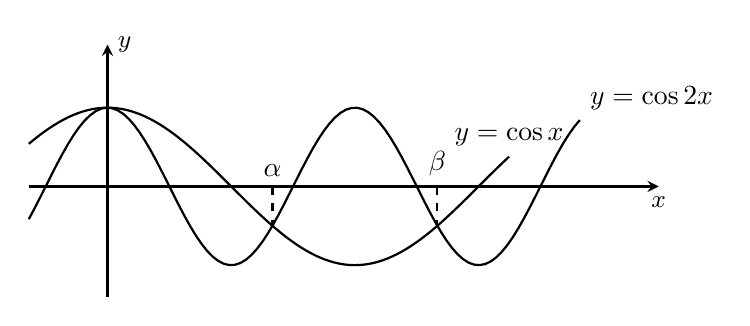
\begin{tikzpicture}[thick,>=stealth,x=1cm,y=1cm,scale=1] 
	\draw[->] (-1,0) -- (7,0) node[below] {\small $x$};
	\draw[->] (0,-1.4)-- (0,1.8) node[right] {\small $y$};
	\draw[thick,samples=100,domain=-1:6] plot(\x,{cos((2*\x)*180/pi)})node[above right] {$y=\cos 2x$};
	\draw[thick,samples=100,domain=-1:5.1] plot(\x,{cos((\x)*180/pi)})node[above] {$y=\cos x$};
	\draw[dashed] (2*pi/3,0)node[above] {$\alpha$}--(2*pi/3,-0.5);
	\draw[dashed] (4*pi/3,0)node[above] {$\beta$}--(4*pi/3,-0.5);
\end{tikzpicture}}
	\loigiai{
		Xét phương trình $\cos 2x = \cos x \Leftrightarrow \hoac{&2x=x+k2\pi\\&2x=-x+k2\pi}\Leftrightarrow \hoac{&x=k2\pi\\&x=\dfrac{k2\pi}{3}} \Leftrightarrow x=\dfrac{k2\pi}{3}$, với $ k \in \mathbb{Z} $.\\
		Suy ra $\alpha =\dfrac{2\pi}{3}$ và $\beta =\dfrac{4\pi}{3}$. Khi đó 
		$$\sin\left(\beta-\alpha \right)=\sin\dfrac{2\pi}{3}\approx 0,87.$$
	}
\end{ex}\cham{10}

\Closesolutionfile{ans}

